\documentclass[11pt,a4paper]{article}
\usepackage[margin=1in]{geometry}
\usepackage[T1]{fontenc}
\usepackage[utf8]{inputenc}
\usepackage{amsmath,amssymb,booktabs,longtable,array,graphicx}
\usepackage{xurl}
\usepackage[round]{natbib}
\usepackage[colorlinks=true,allcolors=blue]{hyperref}
\graphicspath{{../reports/research_story_build/figures/}{../../MNL/experiments/JMP_SEMINAR_SPRINT/figures/}}
\setlength{\emergencystretch}{2em}
% Generated by build_paper_v2_numbers.py from reports/numbers_of_record_v1.json
% and reports/research_story_build/final_descriptives_v1.json. Do not edit values here.
\newcommand{\NSingles}{1,555}
\newcommand{\NCouples}{2,275}
\newcommand{\MinHoursSingles}{6}
\newcommand{\MinHoursCoupleMen}{9}
\newcommand{\MinHoursCoupleWomen}{6}
\newcommand{\CurrentSingleGini}{0.1343}
\newcommand{\CurrentSinglePrefShare}{6.3}
\newcommand{\CurrentSingleEnvShare}{93.7}
\newcommand{\CurrentCoupleGini}{0.1447}
\newcommand{\CurrentCouplePrefPoints}{0.0073}
\newcommand{\CurrentCoupleEnvPoints}{0.1374}
\newcommand{\SingleInterior}{39}
\newcommand{\SingleBounds}{2}
\newcommand{\CoupleFree}{46}
\newcommand{\CoupleInterior}{45}
\newcommand{\CoupleBounds}{1}


\newcommand{\BC}{\operatorname{BC}}
\newcommand{\E}{\mathbb E}
\newcommand{\ind}{\mathbf 1}
\newcommand{\R}{\mathbb R}
\newcommand{\status}{\textit{current-implementation estimate; corrected result pending}}

\title{Unequal Job Opportunities and the Measurement of Well-Being Inequality}
\author{Seminar working paper --- first complete discussion draft}
\date{10 September 2026}

\begin{document}
\maketitle

\begin{abstract}
Random Utility--Random Opportunity (RURO) is a job-choice framework in which
preferences rank employment packages while a separate household-specific
opportunity density governs their availability. We ask how much inequality in
money-metric well-being is associated with unequal job access and earning
opportunities rather than heterogeneous preferences, accounting separately for
non-labour resources and household composition. The empirical applications are
single adults and couples in France. The incremental contribution is to carry an
occupation-augmented RURO structure through tax-benefit pricing, ex-ante
money-metric welfare, and grouped Shapley attribution, then compare it with a
re-estimated common-opportunity model. This is not a claim to invent joint
preference--opportunity estimation. Current estimates were produced by the
sampled-alternatives criterion and unbounded wage density presently implemented.
A corrected estimator, bounded and renormalised wage support, and affected
downstream results are pending; consequently the paper reports those estimates
as provisional evidence and draws no conclusion that requires corrected
magnitudes.
\end{abstract}

\begin{quote}
\textbf{Standing result-status note.}
Verified facts include the source-to-sample reconciliation, the formulas
executed by the historical pipeline, and the current chosen-row-free common
welfare support. Every numerical behavioural or welfare result below is a
current-implementation estimate, not a corrected bounded-support estimate. The
estimator, wage support, parameters, predictions, welfare levels, and
decomposition results are under correction. The corrected resource
classification also makes the earlier nested resource/composition percentages
historical only, so those percentages are withheld. This status follows the
target-model and integrability audit, the sampled-alternatives criterion audit
as qualified by the welfare mission, and the source-to-estimation-sample audit.
WINT-1 establishes that the welfare integrator itself is unaffected by the
chosen-row term: its common support excludes the chosen row, whose contribution
is exactly zero.
\end{quote}

\section{Introduction}

Observed labour supply combines what a household wants with what it can reach.
A worker may choose short hours because time is valuable, because longer-hour
jobs are scarce, or because the available long-hour jobs pay poorly after taxes
and transfers. A non-worker may have a strong preference for work but face a
thin opportunity distribution. Treating all observed differences as tastes
would misdescribe the economic mechanism; treating every non-preference
circumstance as a job opportunity would be equally misleading. Our exhaustive
accounting therefore distinguishes preferences, job access, earning
opportunities, non-labour resources, and household composition or needs.

RURO separates two surfaces. Deterministic utility assigns value to
consumption and leisure. A structural opportunity density assigns relative
availability to employment, hours, occupations, and wages. Extreme-value shocks
then generate probabilistic choice from their product. The distinction matters
for welfare because ex-ante well-being depends on the distribution of potential
jobs, not only on the chosen outcome. It also matters for interpretation:
estimated opportunity densities are neither literal counts of accessible jobs
nor recovered deterministic capability sets.

\subsection{Four strands of literature and the incremental contribution}

The first strand models labour supply as choice among latent jobs. The
Aaberge--Dagsvik--Str\o m tradition combines nonlinear tax schedules with random
job opportunities, and later work studies representations of restricted choice
sets \citep{aaberge1995,aaberge1999,aaberge2009}. Dagsvik and Str\o m develop a
sectoral latent-job formulation, while Dagsvik and Jia make the identification
problem created by unobserved heterogeneity explicit
\citep{dagsvikstrom2006,dagsviketal2014,dagsvikjia2016}. Cap\'eau, Decoster and
Dekkers provide the closest RURO estimation-and-simulation application
\citep{capeau2016}. The present paper inherits joint preference--opportunity
estimation from this literature; its novelty is not the RURO label.

The second strand asks how welfare comparisons can respect heterogeneous
preferences. Equivalent-income methods use a declared reference situation to
map household-specific utility into a common money unit
\citep{dagsvikkarlstrom2005,decosterhaan2015,decancq2015,bargain2013}. Our
cross-sectional object is a level of ex-ante money-metric well-being under a
declared flat-consumption reference, not a reform-specific compensating
variation.

The third strand connects latent jobs to responsibility-sensitive welfare.
\citet{jacquet2026} study a reform comparison for joint-choice couples and ask
how responsibility assignments affect fairness measurement. Our question is
different: cross-sectional inequality in well-being, with singles and couples
as parallel core applications, under one fixed policy system. We do not claim to
implement the full family of measures developed in the separate
Haydar--Maniquet theory project.

The fourth strand attributes nonlinear distributional statistics to inputs.
The Shapley approach averages marginal contributions over orderings
\citep{shorrocks2013}; grouped Shapley--Owen methods preserve a declared
hierarchy among factors \citep{audoly2025}. Here the hierarchy first separates
preferences from all non-preference circumstances, then separates access,
earnings, resources, and composition. Algebraic exhaustiveness does not convert
that allocation into causal identification or a moral-responsibility theorem.

The exact empirical increment is therefore an integrated architecture: an
occupation-augmented RURO model for single and joint couple choices; detailed
tax-benefit pricing; an opportunity-sensitive, preference-respecting money
metric; a grouped distributional attribution; and a re-estimated
common-opportunity comparison. The closest pieces exist separately in the
literature. Their disciplined integration, together with explicit accounting
for what the data do not identify, is the contribution.

\section{Data and institutional setting}

The delivered microdata are the French EUROMOD input file
\texttt{FR\_2016\_a3}. Collection occurred in 2016, while the income reference
year is 2015. The production connector binds that delivery to the
\texttt{FR\_2015} policy system. Amounts entering utility are monthly euros on
the delivery's price scale; wages are euros per hour and labour supply is weekly
hours. Counterfactual monthly gross earnings split ordinary and overtime inputs,
\begin{equation}
Y^{reg}(w,h)=\frac{52}{12}w\min\{h,35\},\qquad
Y^{ot}(w,h)=\frac{52}{12}w\max\{h-35,0\}.
\label{eq:earnings}
\end{equation}
Here $w$ is hourly pay and $h$ is weekly hours. This split is required because
equal total earnings with different hours need not be identical policy inputs.
The budget map is
\begin{equation}
C_i(j)=\max\!\left\{1,
\mathcal B_i^{FR\_2015}\bigl(Y^{reg}(j),Y^{ot}(j),h(j);r_i,d_i\bigr)
\right\},
\label{eq:budget}
\end{equation}
where $r_i$ contains non-labour resources and housing inputs, $d_i$ contains
composition and policy-relevant characteristics, and $C_i(j)$ is disposable
consumption in euros per month after the one-time take-up adjustment. The one
euro floor is a positive-domain modelling device, not a subsistence estimate or
a correction to raw data.

The corrected source audit establishes the EUROMOD connector version, model
root, policy-file digest, and a field-level dictionary for all delivered inputs.
It also establishes that annual employee cash earnings equal twelve times the
calendar-year-average monthly equivalent; multiplying that monthly equivalent
by months worked is incorrect. The hourly wage variable is a predicted or
imputed construction. Positive-income identities hold for most workers, but
some employees have zero recorded employee earnings, so the paper does not call
every wage observed.

\subsection{Parallel samples}

The analysis contains \NSingles{} single-adult households and \NCouples{}
opposite-sex couple households. Both arise from one screen sequence: household
composition; all decision makers aged 20--60; no current education; no relevant
pension status; labour-force status restricted to employee, unemployed, or
inactive; no additional employable or materially earning member; and the final
hours and wage restrictions. These restrictions define the target population.
They are not statements that other households are behaviourally inflexible.

The former ten-hour lift was a processed-data error. In the corrected chosen
rows, minimum positive weekly hours are \MinHoursSingles{} for singles,
\MinHoursCoupleMen{} for couple men, and \MinHoursCoupleWomen{} for couple women.
Values at the seventy-hour cap combine recorded values and projections from
above the cap. Low-hour employees and capped observations therefore require an
explicit observation/support decision before final regeneration.

\begin{figure}[htbp]
\centering
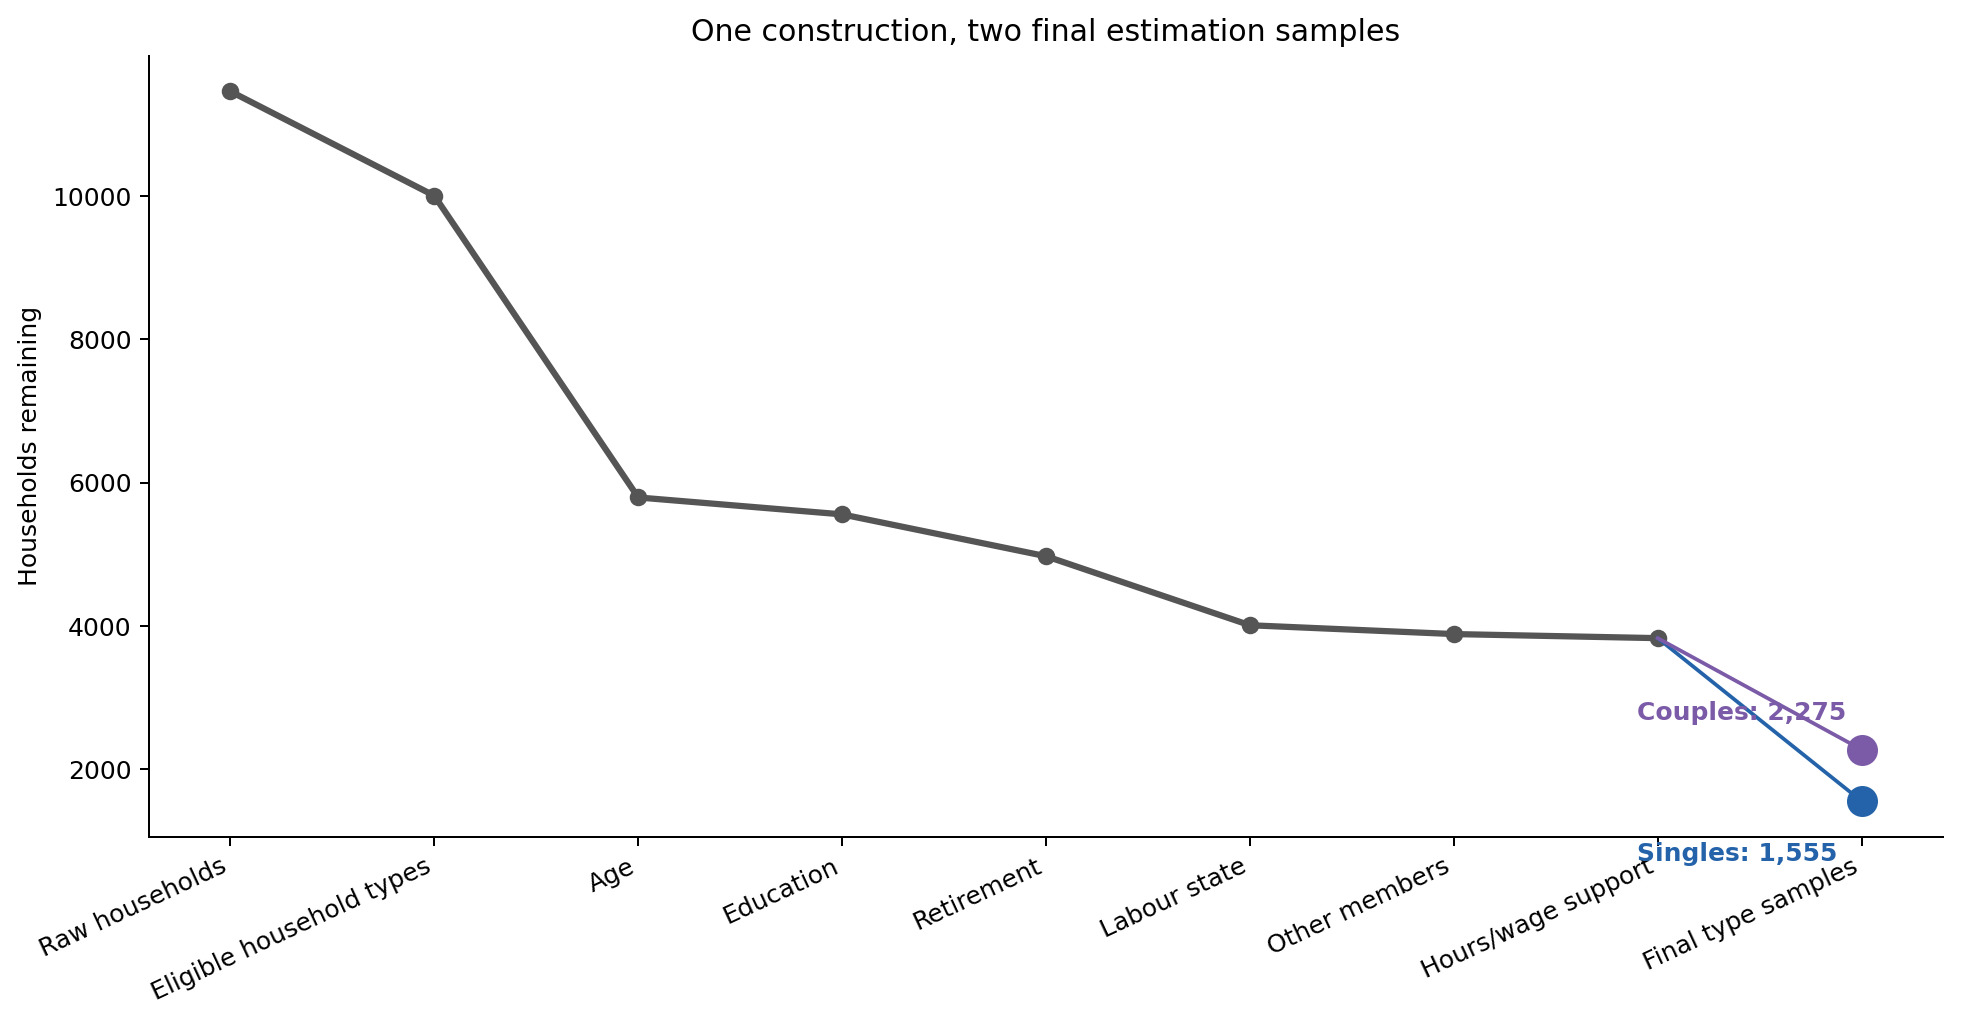
\includegraphics[width=.92\linewidth]{rg_fig1_1_sample_funnel.png}
\caption{Population: delivered French households screened into the final
single-adult and both-flexible couple samples. Units: unweighted household
counts. Measure: observed sample construction. Reference: 2016 delivery,
2015 income year and FR\_2015 policy system. Status: regenerated descriptive
evidence; no model output.}
\label{fig:funnel}
\end{figure}

\begin{figure}[htbp]
\centering
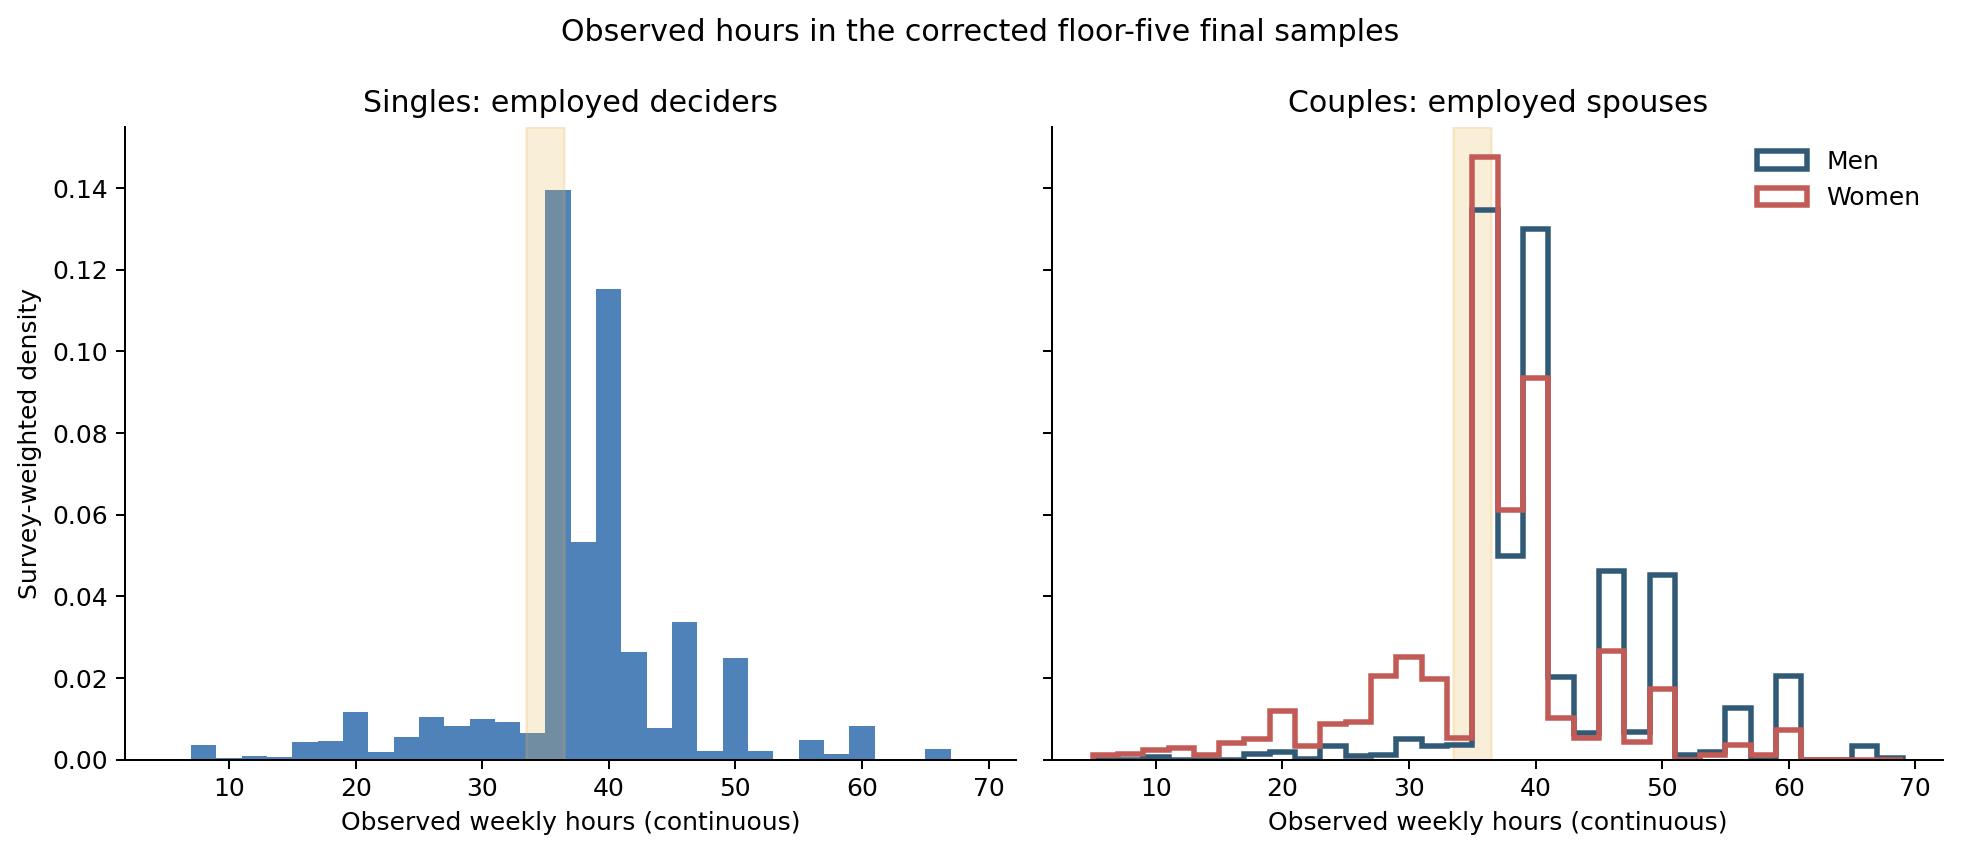
\includegraphics[width=.92\linewidth]{rg_fig2_2_hours_bands.png}
\caption{Population: employed decision makers in the final single and couple
samples. Units: weekly hours. Measure: survey-weighted observed chosen-row
distribution; named structural bands are overlaid for orientation. Reference:
own observed status and hours. Status: regenerated descriptive evidence, not a
model-implied distribution and not evidence of point masses.}
\label{fig:hours}
\end{figure}

\begin{figure}[htbp]
\centering
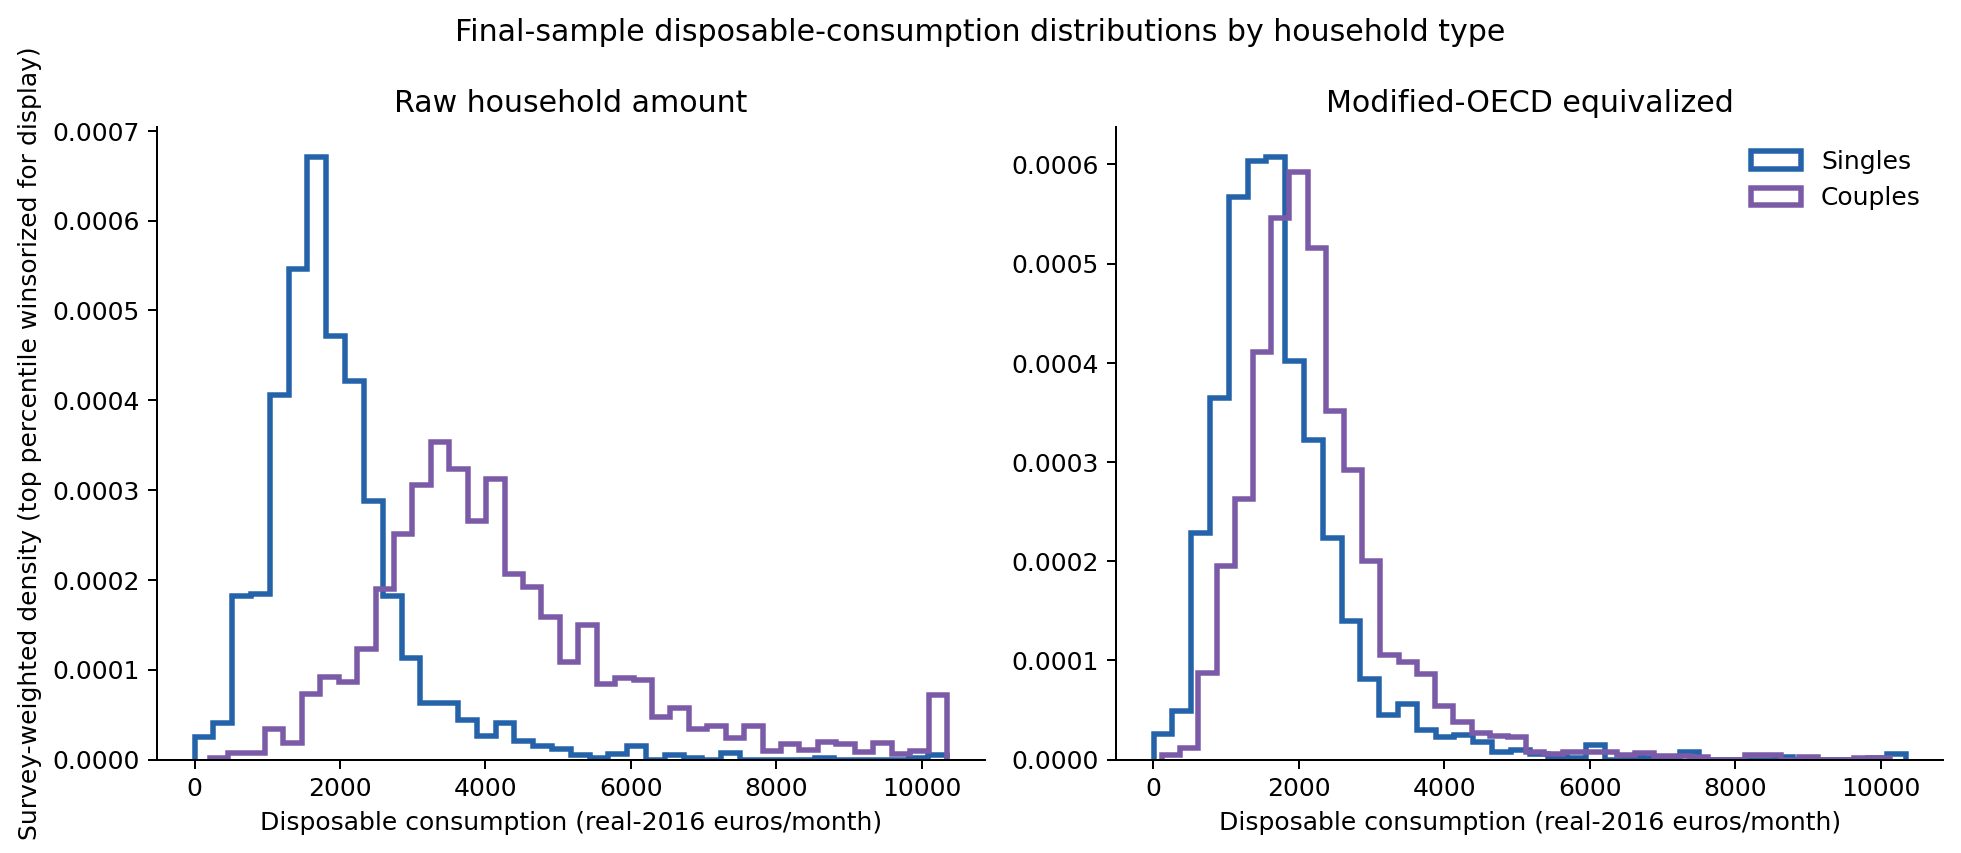
\includegraphics[width=.92\linewidth]{rg_fig2_1_income_distributions.png}
\caption{Population: final single-adult and couple households. Units: monthly
euros, raw and modified-OECD-equivalized as identified in the panels. Measure:
survey-weighted observed chosen-row disposable-consumption distribution.
Reference: actual household composition. Status: regenerated descriptive
evidence; no behavioural or welfare estimate.}
\label{fig:income}
\end{figure}

\paragraph{Calculation, rationale, assumptions, alternative.}
The data stage calculates a decision unit, observed package, policy-priced
budget inputs, and survey-representative descriptives. It is used because joint
choices and nonlinear taxes must be represented at the household level. It
assumes the stated timing, roster links, target-population restrictions, and
one-time take-up imputation. Dropping rather than projecting out-of-support
observations would narrow the population; extending the support would require
valid leisure and wage equations there; an observation or censoring model would
retain the observations but add a new likelihood layer.

\section{Household RURO model, assumptions and identification}

\subsection{Job space and structural choice probabilities}

For a single adult, a working job is $j=(k,h,w)$, with occupation
$k\in\{1,2,3,4\}$, weekly hours $h\in[5,70]$, and hourly wage $w$. Non-employment
is one atom, denoted $0$. The mixed reference measure is
\begin{equation}
\nu=\delta_0+\sum_{k=1}^{4}\delta_k\otimes dh\otimes dw.
\end{equation}
The International Standard Classification of Occupations (ISCO) one-digit
groups are aggregated into four civilian groups: manual/agricultural,
service/sales, clerical, and managerial/professional/technical. ISCO zero lies
outside this recode; the current mode assignment of employed armed-forces cases
is disclosed and remains under decision.

Let $u_i(j;\theta_P)$ be deterministic utility and $g_i(j;\theta_O)$ an
unnormalised structural opportunity density. With iid type-I extreme-value
utility shocks of unit scale,
\begin{equation}
a_i(j;\theta)=u_i(j;\theta_P)+\log g_i(j;\theta_O),\qquad
Z_i^a(\theta)=\int_{\mathcal J_i}e^{a_i(j;\theta)}d\nu(j),
\end{equation}
\begin{equation}
p_i(j;\theta)=\frac{e^{a_i(j;\theta)}}{Z_i^a(\theta)}.
\label{eq:choice}
\end{equation}
For continuous working alternatives $p_i$ is a density relative to $\nu$; at
the atom its value is a probability mass. Density height is not interval mass.

The unbounded historical wage model is not certified for singles with positive
consumption curvature. Under eventual positive-power budget growth on a
positive-measure set of hours, its utility-weighted normalizer diverges. Finite
priced nodes cannot establish the budget at infinity. The initial corrective
candidate is therefore the bounded support $\mathcal W=[2,150]$ euros per hour,
with upper-cap sensitivity at $120$ and $175$. If
$g_i^W(w\mid k)$ is the historical lognormal density, the corrected density is
\begin{equation}
g_i^{W,B}(w\mid k)=
\frac{g_i^W(w\mid k)}{D_i(k;\theta_W)}\ind\{2\leq w\leq w_{max}\},
\end{equation}
\begin{equation}
D_i(k;\theta_W)=
\Phi\!\left(\frac{\log w_{max}-\mu_i(k)}{\sigma}\right)-
\Phi\!\left(\frac{\log 2-\mu_i(k)}{\sigma}\right).
\label{eq:trunc}
\end{equation}
The parameter- and occupation-dependent divisor is part of the economic density
and its derivatives. It is not a numerical sampling adjustment. The support is
a disclosed approximation for a trimmed population, not an identified maximum.
Compact support yields finite normalizers conditional on budgets being bounded
on compact earnings sets and utility remaining on its positive domain.

\subsection{Utility and budgets for singles and couples}

Define the Box--Cox map
\begin{equation}
\BC(x;t)=\begin{cases}(x^t-1)/t,&t\neq0,\\ \log x,&t=0.\end{cases}
\end{equation}
For singles,
\begin{equation}
u_i(j)=\omega_i\BC\!\left(\frac{80-h(j)}{10};\theta_{\ell,g}\right)
+\BC\!\left(\frac{C_i(j)}{1911.108057855561};\theta_c\right),
\label{eq:singleutility}
\end{equation}
\begin{equation}
\omega_i=\beta_{\ell0,g}+\beta_{\ell a,g}a_i
+\beta_{\ell a^2,g}a_i^2+\ind\{g=f\}\beta_{\ell n,g}n_i,
\qquad a_i=(A_i-\bar A_g)/10.
\end{equation}
$A_i$ is age in years and $n_i$ counts all resident household members younger
than twenty. The child coefficient enters additively in the leisure weight; it
is not exponentiated. The leisure weight is not itself a marginal rate of
substitution. The local consumption compensation for leisure depends on both
marginal utilities and the normalization scales.

For a couple, $j=(j_m,j_f)$ and the regimes are neither working, man only,
woman only, and both working. Utility is
\begin{equation}
u_i^C(j_m,j_f)=\omega_{im}\BC(\ell_{im};\theta_{\ell m})
+\omega_{if}\BC(\ell_{if};\theta_{\ell f})
+\log\!\left(\frac{C_i(j_m,j_f)}{3821.448012098882}\right).
\label{eq:coupleutility}
\end{equation}
There is no direct cross-leisure term: $\beta_{\ell\ell}=0$ in the specification
being reported. Spouses are nevertheless dependent through joint choice,
shared consumption, income effects, and nonlinear taxes and transfers.

\begin{table}[htbp]
\centering
\caption{Population: final single-adult and both-flexible couple samples. Units:
utility arguments are dimensionless; money and time units are shown in the
rows. Measure: model specification. Reference: current-implementation model,
with the bounded wage correction pending. Status: structural comparison, not an
empirical result.}
\label{tab:spec}
\begin{tabular}{p{.24\linewidth}p{.32\linewidth}p{.32\linewidth}}
\toprule
Feature & Singles & Couples\\
\midrule
Decision & non-work or one job & joint four-regime package\\
Consumption & decider-only aggregation historically; all-member correction pending & all resident members\\
Consumption curvature & estimated Box--Cox & logarithmic\\
Leisure & one term & spouse-specific additive terms\\
Direct cross-leisure & not applicable & fixed at zero\\
Opportunity factorization & employment, hours, occupation, wage & spouse product conditional on household covariates\\
Dependence in choice & one decision maker & joint budget and joint utility\\
Sampling law & mixed pseudo-random and scrambled-Halton historical panel & joint-regime first, then spouse job coordinates\\
\bottomrule
\end{tabular}
\end{table}

\subsection{Opportunity factors}

Using the uncentred representation, the single-adult working kernel is
\begin{equation}
g_i(k,h,w)=\exp\{E_i+O_{gk}+H_g(h)\}\,g_i^{W}(w\mid k),
\qquad g_i(0)=1.
\label{eq:opp}
\end{equation}
$E_i$ contains the employment intercept, region and urbanization variables,
and $\beta_{E,gsur}(10\,gsur_i)$. Thus a coefficient is applied to ten times
the group unemployment rate; its exponentiated effect is a relative density
factor, not a percentage-point employment effect. $O_{g1}=0$ normalizes the
first occupation group. The hours index has disjoint continuous bands, including
$[33.5,36.5)$ around thirty-five hours. It changes density height across an
interval; it is not an atom at thirty-five hours. For example, the integrated
mass of band $b$ is its width times $e^{\beta_b}$ divided by the hours
normalizer.

For couples the uncentred opportunity kernel factors as
$g_i^C(j_m,j_f)=g_{im}(j_m)g_{if}(j_f)$. This conditional factorization does not
imply independent decisions, because equation~\eqref{eq:coupleutility} and the
joint budget enter the same choice probability.

\paragraph{Identification.}
Preferences and opportunities enter $a_i$ additively. Their separation relies
on functional form, observed variation, and exclusion restrictions: local group
unemployment, region and urbanization are assigned to access and excluded from
preferences; demographic shifters enter declared preference or wage channels.
The design does not nonparametrically recover capability sets, discrimination,
amenities, or persistent unobserved heterogeneity. Sorting can invalidate a
causal reading of geography. A benchmark comparison tests the consequences of a
common density; it does not identify the preferred model.

\paragraph{Calculation, rationale, assumptions, alternative.}
The model calculates the probability density in equation~\eqref{eq:choice} from
utility and availability. It is used to avoid forcing restricted choices into
tastes. It requires a proper mixed support, finite normalizers, valid channel
exclusions, and unit-scale extreme-value shocks. A common-menu random-utility
model is a coherent benchmark but removes household-specific access. A richer
nonparametric opportunity process would weaken functional-form assumptions but
requires new identifying variation and much denser data.

\section{Estimation and numerical implementation}

\subsection{Structural density, choice probability, and proposal density}

The structural opportunity density $g_i$ is economic. The choice density $p_i$
combines $g_i$ with utility. The numerical proposal $q_i$ is chosen by the
researcher to place simulated alternatives; it is not an opportunity density.
For a stochastic single-adult draw,
\begin{equation}
q_i(j)=q_E(e)\bigl[q_O(k\mid dgn_i,educ3_i)q_H(h)q_W(w\mid i,k)\bigr]^e.
\end{equation}
$q_H$ is the exact marginal sum over overlapping mixture components. For
couples the proposal first samples a joint participation regime and then samples
the job coordinates of each working spouse. The current wage coordinate uses a
scrambled Halton point set and is dependent within household.

\subsection{Historical criterion and authorized correction}

Let $j_i^*$ be the observed package, $x_{ir}$ stochastic alternatives, and
$a_i=u_i+\log g_i$. The historically implemented criterion is
\begin{equation}
\ell_i^C(\theta)=a_i(j_i^*;\theta)-
\log\!\left[e^{a_i(j_i^*;\theta)}+
\sum_{r=1}^{R}\frac{e^{a_i(x_{ir};\theta)}}{q_i(x_{ir})}\right].
\label{eq:hybrid}
\end{equation}
It combines a unit-weight chosen row with importance-weighted stochastic rows.
The criterion audit establishes that this is a finite-$R$ approximation to a
direct simulated population log-density, carrying an additional chosen-row
term of order $R^{-1}$. It is not the exact conditional sampled-alternatives
likelihood. The estimates reported below were obtained from
equation~\eqref{eq:hybrid}; they are not relabelled as corrected.

The authorised successor regenerates iid joint alternatives. For a sampled
multiset $D_i$ and multiplicity $n_y$, iid factorization gives
\begin{equation}
\Pr(y\text{ chosen}\mid D_i)=
\frac{n_y\exp\{a_i(y)-\log q_i(y)\}}
{\sum_{z\in D_i}^{slots}\exp\{a_i(z)-\log q_i(z)\}}.
\label{eq:conditional}
\end{equation}
The chosen package receives the same $-\log q_i$ correction as every other
candidate, and repeated atoms retain multiplicity. The conditional likelihood
is exact for its stated sampling experiment. That statement does not imply an
unbiased finite-sample maximizer, exact coverage, or no benefit from enlarging a
sampled menu. The current scrambled-Halton wage panel is not iid and cannot be
made iid by changing stored corrections. It must be regenerated. Whether pilot
proposal parameters are independent of the observed-choice sample, or instead
must be cross-fitted, remains unresolved.

For population prediction and welfare, the relevant numerical object is direct
integration of the structural population kernel. A generic importance estimate
on working draws is
\begin{equation}
\widehat Z_i^a=e^{a_i(0)}+\frac{1}{R}\sum_{r:x_{ir}\neq0}
\frac{e^{a_i(x_{ir})}}{q_i(x_{ir})}.
\label{eq:direct}
\end{equation}
The chosen package is an evaluation point in the numerator and is absent from
this denominator. The atom and working integral must be scaled coherently; the
$1/R$ cannot be removed from only one limb.

\subsection{Inference and weights}

Household-cluster-robust inference aggregates one score per household, permits
arbitrary dependence among that household's simulated rows, and assumes
independence across households. For interior coordinates $\theta_I$,
\begin{equation}
s_i=\frac{\partial\ell_i}{\partial\theta_I},\qquad
\widehat{\operatorname{Var}}_{CR1}(\hat\theta_I)=
\frac{G}{G-K_I}H^{-1}\left(\sum_{i=1}^{G}s_is_i'\right)H^{-1},
\label{eq:cr1}
\end{equation}
where $G$ is the number of households, $K_I$ the number of interior coordinates,
and $H$ the negative Hessian. The factor $G/(G-K_I)$ is the adopted CR1
finite-sample adjustment. Active-bound coordinates require constrained or
one-sided treatment; ordinary symmetric intervals are not reported for them.
The current singles fit has \SingleInterior{} interior and \SingleBounds{}
active-bound coordinates; the couples fit has \CoupleFree{} free,
\CoupleInterior{} interior, and \CoupleBounds{} active-bound coordinates.

Survey weights make descriptive, fit, and welfare aggregates represent the
target population. They do not enter the unweighted estimation objective.
Conditional parameter uncertainty propagates equation~\eqref{eq:cr1} while
holding the data, model, active set, policy build, numerical integration design,
and welfare reference fixed. It is not numerical integration error and it is not
normative-reference sensitivity.

\paragraph{Calculation, rationale, assumptions, alternative.}
Estimation calculates parameters from conditional sampled-menu probabilities;
population prediction calculates equation~\eqref{eq:direct}. Separating these
operations keeps one economic model while respecting two numerical questions.
The conditional estimator requires iid joint draws, positive proposal support,
correct multiplicities, and an independent or properly treated pilot proposal.
Keeping the current dependent point set licenses direct integration, not the
iid conditional factorization. A direct simulated maximum-likelihood estimator
would retain the point set but has finite-integration bias and must treat the atom
and normalization coherently.

\section{Money-metric well-being and inequality decomposition}

\subsection{From opportunities to ex-ante value}

For a coalition $S$ of equalized factors, distinguish three objects:
\begin{equation}
G_{i,S}=\int_{\mathcal J}\widetilde g_{i,S}(j)d\nu(j),\qquad
Z_{i,S}=\int_{\mathcal J}e^{u_{i,S}(j)}\widetilde g_{i,S}(j)d\nu(j),
\end{equation}
\begin{equation}
J_{i,S}=\frac{Z_{i,S}}{G_{i,S}}=
\int_{\mathcal J}e^{u_{i,S}(j)}\widehat g_{i,S}(j)d\nu(j),qquad
V_{i,S}=\log J_{i,S},
\label{eq:value}
\end{equation}
where $\widehat g_{i,S}=\widetilde g_{i,S}/G_{i,S}$. $G$ is opportunity mass,
$Z$ is a utility-weighted normalizer, and $J$ is their normalized ratio. No one
symbol is used for all three. The calculation is ex ante: latent jobs are
averaged before the logarithm and monetary inversion. Observed non-employment
does not remove working opportunities from this integral.

Randomized quasi-Monte Carlo (RQMC) uses randomized, deliberately well-spread
points for the latent-job integral. On scramble $r$ with $M$ common-support
nodes,
\begin{equation}
\widehat J_{i,S,r}=\frac1M\sum_{m=1}^{M}
\exp\{u_{i,S}(J_{irm})+\log\widehat g_{i,S}(J_{irm})
-\log q_r(J_{irm})\},
\end{equation}
\begin{equation}
\overline J_{i,S}=\frac1K\sum_{r=1}^{K}\widehat J_{i,S,r},
\qquad \widehat V_{i,S}=\log\overline J_{i,S}.
\label{eq:rqmc}
\end{equation}
Averaging occurs before the logarithm and before inversion. WINT-1 follows the
executed call path and finds no observed row on this common support. Therefore
the chosen-row contribution to equations~\eqref{eq:rqmc} is exactly zero. The
support must still match the corrected structural density; reusing priced nodes
outside the new support requires zero target contribution with the original
proposal weight, not division by a random retained-node count.

\subsection{Monetary inversion}

Remove the consumption term from attained utility,
\begin{equation}
L_{i,S}(j)=u_{i,S}(j)-
\BC(C_{i,S}(j)/\lambda_c;\theta_{c,S}),
\end{equation}
and define the reference map
\begin{equation}
\Phi_{i,S}(m)=\log\int_{\mathcal J}
\exp\!\left\{L_{i,S}(j)+\BC(m/\lambda_c;\theta_{c,S})\right\}
\widehat g_{i,S}(j)d\nu(j).
\label{eq:phi}
\end{equation}
Money-metric well-being $W_{i,S}$ is the unique monthly euro amount satisfying
\begin{equation}
\Phi_{i,S}(W_{i,S})=V_{i,S}.
\label{eq:invert}
\end{equation}
The same flat disposable-consumption amount is inserted at every reference
alternative, including non-employment. It replaces consumption in the
comparator; it does not replace hourly wages, rerun EUROMOD, or remove the effect
of actual earnings on attained value. Both sides use the same coalition's
preferences, opportunity density, and non-consumption utility. Existence and
uniqueness require a continuous, strictly increasing reference map over the
permitted monetary bracket and finite positive normalizers. A one-hundred-euro
difference means a one-hundred-euro monthly difference in the flat reference
consumption needed to match attained ex-ante value; it is not necessarily a
cash-transfer equivalent under the actual nonlinear budget.

\subsection{Interpersonal comparison, equivalization, and inequality}

The welfare unit is the modelled household. Survey weighting also occurs at the
household level. Couples are unitary decision makers in this application; the
model does not identify within-household allocation. The modified-OECD scale is
\begin{equation}
m_i^{OECD}=1+0.5(N_{i,14+}-1)+0.3N_{i,<14},
\end{equation}
and equivalized welfare is $W_{i,S}/m_{i,S}^{OECD}$. The scale moves with the
composition factor so the counterfactual state is internally coherent. Closure
is a consequence of this choice, not its ethical justification. Raw household,
equivalized household, and pooled individual comparisons answer different
questions and are not forced to coincide with type-specific constants.

With normalized household survey weights $\omega_i$, the implemented Gini is
\begin{equation}
I(S)=\frac{\sum_i\sum_j\omega_i\omega_j
|W_{i,S}-W_{j,S}|}{2\sum_i\omega_iW_{i,S}},
\qquad \sum_i\omega_i=1.
\label{eq:gini}
\end{equation}
An income Gini and a money-metric well-being Gini differ because the latter
includes preferences, leisure, and opportunity distributions. Atkinson or
generalized-entropy indices would make inequality aversion or subgroup
decomposability more explicit; they would change the social summary, not the
underlying household welfare values. No uncomputed index is reported as a result.

\subsection{Factor operators and grouped attribution}

The factors are $P$ (preferences), $A$ (employment, hours, and occupation
access), $B$ (wage-offer or earning opportunities), and $D$ (resources and
composition/needs). Each operator substitutes declared reference primitives
before normalizing the opportunity kernel and recomputing budgets, welfare,
equivalence scales, and inequality. $q$ and normalizers are numerical or derived
objects, not separate economic factors. The corrected four-field resource
classification and the treatment of job-history counters must be resolved before
the $D$ states are repriced.

For the first-level two-player table, let one mean equalized and let $I^{ab}$ be
inequality with preference status $a$ and environment status $b$. One-factor
equalization effects are $I^{00}-I^{10}$ and $I^{00}-I^{01}$. They are not
Shapley contributions. The two-player Shapley allocation is
\begin{equation}
C_P=\tfrac12[(I^{00}-I^{10})+(I^{01}-I^{11})],\qquad
C_E=\tfrac12[(I^{00}-I^{01})+(I^{10}-I^{11})].
\label{eq:twoplayer}
\end{equation}
It averages each marginal effect over both positions in an ordering and thereby
allocates the interaction.

Inside $E=\{A,B,D\}$, the executed grouped rule is
\begin{equation}
C_i=\sum_{Q\in\{\varnothing,\{P\}\}}\frac12
\sum_{T\subseteq E\setminus\{i\}}
\frac{|T|!(2-|T|)!}{3!}
\left[I(Q\cup T)-I(Q\cup T\cup\{i\})\right],
\quad i\in E.
\label{eq:owen}
\end{equation}
Contributions may be negative. Shares sum to the reducible difference between
baseline and the fully equalized state; they sum to baseline inequality only if
the fully equalized state has zero inequality. Neither closure nor the ordering
rule identifies causal responsibility.

\paragraph{Calculation, rationale, assumptions, alternative.}
This stage calculates normalized ex-ante value, inverts it into monthly euros,
measures its weighted inequality, and allocates the reducible difference across
factors. It is used because chosen income alone omits leisure and opportunity
variation while a raw utility index is not interpersonally comparable. It
requires finite integrals, a monotone reference map, the unitary-household
assumption for couples, a declared equivalence scale, and coalition operators
that alter only their assigned primitives. Ex-post welfare, common-reference
opportunities, compensating variation, another inequality index, or flat rather
than grouped Shapley attribution would each answer a different normative
question.

\section{Behavioural and welfare evidence for singles and couples}

\subsection{Parameter interpretation and fit}

The current coefficients are estimates of equation~\eqref{eq:hybrid}. The
female singles child coefficient is an additive change in $\omega_i$, not an
exponentiated multiplicative effect. The group-unemployment coefficient applies
to $10\,gsur_i$. Hours-band coefficients compare density heights, and the narrow
thirty-five-hour band is continuous. Mean desired hours do not establish an
every-worker claim. The external wish-to-work-more variable lacks an established
coding direction, so no directional robustness conclusion is drawn from it.

Fit is evaluated by population probabilities from the structural model, not by
conditional sampled-menu probabilities. Singles and couples are both core:
couple fit uses the four joint participation regimes and spouse-specific hours,
occupation, and wage margins. A fit comparison is external benchmarking unless
the identifying argument itself uses that source. Public aggregate wage and
hours benchmarks do not turn the model's structural exclusions into identified
causal effects.

\subsection{Provisional welfare evidence}

\begin{table}[htbp]
\centering
\caption{Population: final single-adult and both-flexible couple samples. Units:
Gini points and percentage share where marked. Measure: model-implied raw
household money-metric well-being and first-level grouped attribution. Reference:
the current paper's primary welfare reference. Status: current-implementation
estimates under equation~\eqref{eq:hybrid} and the historical unbounded wage
density; corrected results pending.}
\label{tab:provisional}
\begin{tabular}{lcc}
\toprule
Quantity & Singles & Couples\\
\midrule
Baseline raw well-being Gini & \CurrentSingleGini{} & \CurrentCoupleGini{}\\
Preference attribution & \CurrentSinglePrefShare\% & \CurrentCouplePrefPoints{} points\\
Non-preference attribution & \CurrentSingleEnvShare\% & \CurrentCoupleEnvPoints{} points\\
\bottomrule
\end{tabular}
\end{table}

The provisional evidence points toward a large role for non-preference
circumstances in both populations. That qualitative pattern is useful for
motivating the corrected analysis, but the corrected magnitude, factor ordering,
and statistical comparison cannot yet be drawn. The nested access, earnings,
resources, and composition percentages are not reproduced because the corrected
field classification requires repricing. Couples are not relegated to future
work: their joint model, sample, fit targets, welfare construction, and pending
correction are part of the same empirical argument.

Actual non-workers are included in ex-ante integration over working and
non-working alternatives. Their opportunities therefore affect welfare even
when the chosen state is non-employment. Reference flattening applies only to
the comparator in equation~\eqref{eq:phi}; actual earnings opportunities remain
in equation~\eqref{eq:value}.

\subsection{Numerical, parameter, and reference uncertainty}

For a fully recomputed scalar $T$, a leave-one-scramble-out jackknife omits one
entire independent scramble, reruns averaging, inversion, equivalization, Gini,
and attribution, and measures integration variability. If there are $K$
scrambles,
\begin{equation}
\bar T_{(-)}=K^{-1}\sum_rT_{(-r)},\qquad
se_{jack}=\left[\frac{K-1}{K}\sum_r(T_{(-r)}-\bar T_{(-)})^2\right]^{1/2}.
\end{equation}
This is numerical integration uncertainty. Conditional parameter intervals
propagate equation~\eqref{eq:cr1}. Reference sensitivity changes a normative
input to equations~\eqref{eq:phi}--\eqref{eq:invert}. The three are reported
separately. No wider reference range is called a confidence interval, and no
narrow RQMC band is evidence that parameter uncertainty is small.

\section{Comparisons and sensitivity}

\subsection{Common-opportunity random-utility model}

The common-opportunity comparison replaces every household-specific density by
one normalized density,
\begin{equation}
\bar g(0)=\pi_0,\qquad
\bar g(1,k,h,w)=\pi_1\bar p(k)p_H(h)
\phi_{LN}(w\mid\bar\mu(k),\widehat\sigma),
\end{equation}
with $\pi_0+\pi_1=1$ and each conditional component integrating or summing to
one. It does not set $g$ to zero, which would remove alternatives. Taste terms
are re-estimated under the restriction. The recorded criterion difference is
not a likelihood-ratio test because surviving opportunity coefficients were
held at the RURO values rather than freely re-optimized. It is descriptive
benchmark evidence, not formal identification.

\subsection{Geography and external comparison}

Geographic attribution changes the location-related limb of current employment
access. It is therefore conditional on the model's channel assignment. It is
not a lower bound on the total importance of place: omitted wage, hours,
amenity, migration, and sorting channels may offset or reinforce it. Comparisons
with other countries or papers require matching the population, welfare unit,
numerator, denominator, policy question, and reference environment. Percentages
from reform compensating variation are not directly comparable to shares of
cross-sectional well-being inequality.

\begin{figure}[htbp]
\centering

\includegraphics[width=0.96\linewidth]{figE1_matched_pair.png}
\caption{\textbf{Similar estimated preferences, different employment-access
environments.} The two single men are selected by the stated matching rule
among employed households in the same observed occupation group, hours band
and wage quintile. Their estimated leisure-preference curves are close, not
identical. Panel (a) plots the leisure component of utility; panels (b) and (c)
show the specified opportunity masses over hours and occupations; panel (d)
shows conditional wage-offer densities and marks the observed wages. In this
same-sex comparison the hours and occupational profiles are common conditional
on employment, so their unconditional mass differences are driven primarily by
the employment-access margin. The example illustrates a model-conditional
contrast, not a causal regional effect, an individual ability ranking or a
recovered count of available jobs. Population: two anonymized employed single
men in occupation group 4, a common hours band, and observed-wage quintile 4.
Units: weekly hours and euros per hour. Measure: utility component and
opportunity mass/density, not choice probability. Reference: each household's
estimated profile under the current implementation. Status: model-implied
diagnostic; corrected estimator and support results pending.}
\label{fig:matched-pair}
\begin{minipage}{0.96\linewidth}\footnotesize
\textit{Note:} The forward rule restricts preference distance to the lowest
decile of admissible distances and maximizes total-variation opportunity
distance, subject to the displayed clean-separation threshold. The pair is
matched on occupation group, hours band and wage quintile; neither preferences
nor observed job bundles are asserted to be identical.
\end{minipage}
\end{figure}

\section{Limitations and conclusion}

The first limitation is computationally immediate: the corrected estimator,
wage support, and downstream results do not yet exist. Second, bounded wage
support is a disclosed structural approximation, not an identified supremum;
its cap sensitivity and budget coverage must be reported. Third, the target
population excludes same-sex couples, older or studying decision makers,
households with additional employable adults, and workers outside the retained
support. Fourth, geography is not causal. Fifth, opportunity factors are
parametric densities rather than literal choice sets. Sixth, the couple model is
unitary and fixes direct cross-leisure interaction to zero. Seventh, the
one-euro consumption floor and seeded take-up traits are modelling assumptions.
Eighth, the resource/composition partition still requires decisions on
job-history counters and non-cash benefits. Ninth, the current data do not
establish persistent unobserved heterogeneity merely because attempted
extensions were weakly recovered.

The paper's substantive claim is therefore deliberately narrower than a final
percentage. Unequal employment, hours, occupation, and wage opportunities are
economically distinct from preferences and can matter for ex-ante well-being
even when chosen outcomes look similar. Resources and household composition are
separate non-preference channels needed for exhaustive accounting. The current
implementation suggests these distinctions matter for singles and couples, but
corrected magnitudes await the authorized refit and downstream regeneration.

\appendix

\section{Reproducibility map}

The canonical research notebook is
\path{MNL/experiments/JMP_SEMINAR_SPRINT/JMP_research_lab.ipynb}. It
exposes authenticated frames and cached draws, replays the current criterion,
loads inference and fit outputs, and dispatches cached welfare and figure stages.
Raw survey construction, arbitrary fresh alternative generation, EUROMOD
repricing, and external benchmark construction remain external stages. Engine
capability, the package actually selected by the notebook, and device evidence
are separate facts. The local parity record compares Torch on CPU with JAX for
the final singles model and reports CUDA unavailable on that machine. A CUDA
profile exposed by the engine is therefore not a measured local CUDA result,
and no singles result establishes couples device support.

The corrective sources are
\path{MNL/docs/corr/target_model_and_integrability_v1.md},
\path{MNL/docs/jmp_methodology/JMP_sampled_alternatives_criterion_audit_v1.md},
\path{MNL/docs/corr/fr2016_source_to_estimation_sample_audit_v1.md}, and
\path{Job_Market_paper/reports/model_extraction_v1.md}. The source audit's
field dictionary and machine-readable evidence supply units, policy identifiers,
and sample counts. Empirical numerals in this manuscript are generated from
\path{reports/numbers_of_record_v1.json} and the regenerated final
descriptives registry by \path{manuscript/build_paper_v2_numbers.py}.

\section{Pending substantive calculations and decisions}

\begin{enumerate}
\item Generate iid joint alternatives; establish independent or cross-fitted
pilot proposals; implement equation~\eqref{eq:conditional}; and re-estimate
singles and couples.
\item Implement equations~\eqref{eq:trunc} in estimation, derivatives,
prediction, and welfare; price uncovered nodes; and run the stated upper-cap
sensitivity. The old unbounded singles normalizer is not unconditionally
certified because finite pricing does not establish budget growth at infinity.
\item Aggregate all resident-member disposable resources for singles, retain
the full accounting outputs, and re-estimate.
\item Decide the observation model for employed hours outside the support and
the treatment of employed ISCO-zero decision makers.
\item Finalize economic factor allocation for job-history counters and non-cash
benefits; then reprice the corrected resource/composition states. Until then the
nested percentages cannot be interpreted.
\item Recompute parameters, population fit, welfare, uncertainty, and grouped
attribution for both household types. No corrected component ranking is yet
available.
\end{enumerate}

\bibliographystyle{plainnat}
\bibliography{JMP_working_paper_for_seminar_v2}

\end{document}
